\documentclass[10pt]{extarticle}
\usepackage[a4paper,margin=1.5cm,columnsep=0.7cm]{geometry}
\usepackage{amsmath,amssymb}
\usepackage{graphicx}
\usepackage{enumitem}
\usepackage{booktabs}
\usepackage{array}
\usepackage{tabularx}
\usepackage[T1]{fontenc}
\usepackage{multicol}

\setlength{\parindent}{0pt}
\setlength{\parskip}{4pt}
\renewcommand{\arraystretch}{1.15}

\newenvironment{qoptions}{\begin{itemize}[leftmargin=1.8em,itemsep=2pt,topsep=2pt,label={}]}{\end{itemize}}
\newcommand{\opt}[2]{\item[({#1})] {#2}}

\newcommand{\sectionhdr}[1]{\par\vspace{4pt}\noindent\textbf{\large #1}\par\vspace{2pt}}
\newcommand{\subsectionhdr}[1]{\par\vspace{3pt}\noindent\textbf{#1}\par\vspace{2pt}}

\pagestyle{empty}

\begin{document}
\begin{center}
{\LARGE\bfseries JEE (Main+Advanced) Score-II --- Test 37 (10 Feb 2025)}
\end{center}
\vspace{6pt}

\begin{multicols}{2}

\sectionhdr{PART-1: PHYSICS}
\subsectionhdr{Section-I (i): One or more correct}

\textbf{1.} In the circuit shown, all voltmeters are identical but ammeters are non-identical. The reading of A$_1$ and A$_2$ are 5 mA and 4.7 mA respectively. Reading of voltmeter connected across PQ is 9 volts.

\begin{center}
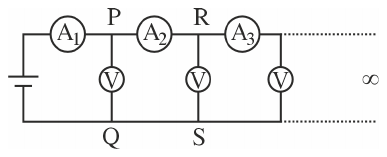
\includegraphics[width=0.9\linewidth]{Score-II - Test 37 (10 Feb 2025)-img/p1phy_q1_circuit.png}
\end{center}

\begin{qoptions}
\opt{A}{Sum of the reading of all voltmeters is 150 volts.}
\opt{B}{Sum of the reading of all voltmeters is 90 volts.}
\opt{C}{Resistance of voltmeter is 18 k$\Omega$}
\opt{D}{Resistance of voltmeter is 30 k$\Omega$}
\end{qoptions}

\textbf{2.} $\text{Tc}_{43}^{99}$ radio-nuclide decays by $\gamma$-emission with a half-life of 6 hours and by $\beta$-emission with a half-life of $2.12\times10^5$ years. A small quantity of solution containing $\text{Tc}_{43}^{99}$ with an activity of 1.0 $\mu$Ci (micro Curie) is injected into the blood stream of an adult person. The solution mixes rapidly and uniformly in the person's blood. It is excreted from the kidneys with an effective half-life of 6 hours. A 1 ml sample of the blood taken after 3.0 hours reveals an activity of 3.70 disintegrations per second on an average. (Note:- 1 Ci (Curie) = $3.70\times10^{10}$ disintegrations per second).

\begin{qoptions}
\opt{A}{Decay constant $\lambda_k$ for excretion from kidney is 0.12 hr$^{-1}$}
\opt{B}{Decay constant $\lambda_k$ for excretion from kidney is 0.6 hr$^{-1}$}
\opt{C}{Volume of blood in person's body is 5 liter}
\opt{D}{Volume of blood in person's body is 6 liter}
\end{qoptions}

\textbf{3.} Three small identical neutral metal balls are at the vertices of an equilateral triangle. The balls are in turn connected to an isolated large conducting sphere whose centre is on the perpendicular erected from the plane of the triangle and passing through its centre. As a result the first and second balls have acquired charges q$_1$ and q$_2$ respectively. If q$_1$ = 4$\mu$C, q$_2$ = 3$\mu$C, then the charge q$_3$ in $\mu$C is (Assume that charge distributions of any ball or sphere remains uniform)

\begin{qoptions}
\opt{A}{2 $\mu$C}
\opt{B}{3 $\mu$C}
\opt{C}{2.25 $\mu$C}
\opt{D}{1.25 $\mu$C}
\end{qoptions}

\textbf{4.} A uniform rod AB of mass M is attached to a hinge at one end A, and released from rest from the horizontal position. The rod rotates about A, and when it reaches the vertical position the rod strikes a sphere of mass m and radius r initially at rest on the smooth horizontal surface as shown in the adjacent figure. The impact is along the horizontal direction and perfectly elastic. If at the moment of impact the lowest end of the rod is very close to the smooth horizontal surface. After the impact, the sphere moves along the horizontal and the rod, subsequently rises to a maximum of 60\textdegree\ with the vertical. Choose the correct statement(s) from the following, taking into account the information given above. The length of the rod equals $\sqrt2r$. $\left(r=\dfrac{6\sqrt2}{10}\text{m}\right)$.

\end{multicols}
\begin{center}
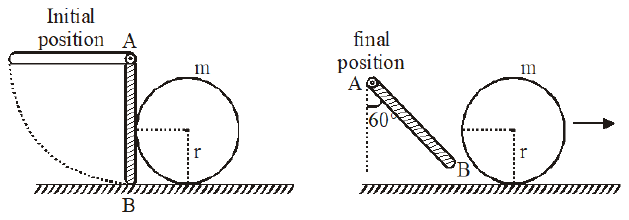
\includegraphics[width=0.55\linewidth]{Score-II - Test 37 (10 Feb 2025)-img/p1phy_q4_rodsphere.png}
\end{center}
\begin{multicols}{2}

\begin{qoptions}
\opt{A}{The ratio $\dfrac Mm$ is $\dfrac32$}
\opt{B}{The ratio $\dfrac Mm$ is $\dfrac23$}
\opt{C}{The speed of the sphere just after collision is 6 m/s}
\opt{D}{The speed of the sphere just after collision is 3 m/s}
\end{qoptions}

\textbf{5.} Figure below shows four lines OA, OB, OC, OD (representing various processes such as isothermal, adiabatic, isobaric for a monoatomic and a diatomic ideal gas) on a work done by the gas (W) versus heat supplied (Q) graph. The initial states of both the gases are the same and so also the scales for the two axes.

\begin{center}
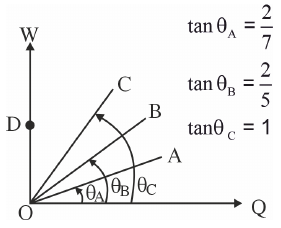
\includegraphics[width=0.9\linewidth]{Score-II - Test 37 (10 Feb 2025)-img/p1phy_q5_gasgraph.png}
\end{center}

\begin{qoptions}
\opt{A}{OA represents isobaric process for diatomic gas}
\opt{B}{OB represents isobaric process for diatomic gas}
\opt{C}{OC represents isothermal process for diatomic gas}
\opt{D}{OD represents adiabatic process for diatomic gas}
\end{qoptions}

\textbf{6.} A point object is placed at 30 cm from a convex glass lens $\left(\mu_s=\dfrac32\right)$ of focal length 20 cm. The final image of object will be formed at infinity if

\begin{qoptions}
\opt{A}{Another concave lens of focal length 60 cm is placed in contact with the previous lens}
\opt{B}{Another convex lens of focal length 60 cm is placed at a distance of 30 cm from the first lens}
\opt{C}{The whole system is immersed in a liquid of refractive index 4/3}
\opt{D}{The whole system is immersed in a liquid of refractive index 9/8}
\end{qoptions}

\subsectionhdr{Section-I (ii): Single Correct}

\textbf{Paragraph for Questions 7 and 8}

Consider the Bohr model of hydrogen atom. let m$_e$ and e be the mass and magnitude of the charge of the electron respectively. Let a$_0$ be the ground state radius (Bohr radius)

\textbf{7.} Consider a two electron system with atomic number Z = 4. use the Bohr model to obtain the ground state radius r. If $r=\dfrac{ya_0}3$, then the value of y is (Assume the two electrons are in the same circular orbit (n = 1) and as far apart as possible)

\begin{qoptions}
\opt{A}{0.12}
\opt{B}{0.40}
\opt{C}{0.80}
\opt{D}{None}
\end{qoptions}

\textbf{8.} The first ionization energy $I_2^{th}$ of the two electron system for Z = 4 is given as $I_2^{th}=\alpha I_H$, the value of $\alpha$ is (if $I_H$ is ionization energy of hydrogen atom)

\begin{qoptions}
\opt{A}{21.7}
\opt{B}{24.25}
\opt{C}{12.125}
\opt{D}{6.125}
\end{qoptions}

\textbf{Paragraph for Questions 9 and 10}

Figure shows how the resistance of a resistor and the reactances of an inductor and a capacitor vary with angular frequency $\omega$. Resistance R is independent of frequency, while the reactances X$_L$ and X$_C$ are not. If $\omega=0$, corresponding to a dc circuit, there is no current through a capacitor because $X_C\to\infty$, and there is no inductive effect because $X_L=0$. In the limit $\omega\to\infty$, $X_L$ also approaches infinity, and the current through an inductor becomes vanishingly small; recall that the self-induced emf opposes rapid changes in current. In this same limit, $X_C$ and the voltage across a capacitor both approach zero.

Figure shows an application of the above discussion to a loudspeaker system. Low-frequency sounds are produced by the woofer, which is a speaker with large diameter; the tweeter, a speaker with smaller diameter, produces high frequency sounds. In order to route signals of different frequency to the appropriate speaker, the woofer and tweeter are connected in parallel across the amplifier output. The capacitor in the tweeter branch blocks the low-frequency components of sound but passes the higher frequencies; the inductor in the woofer branch does the opposite.

\end{multicols}
\begin{center}
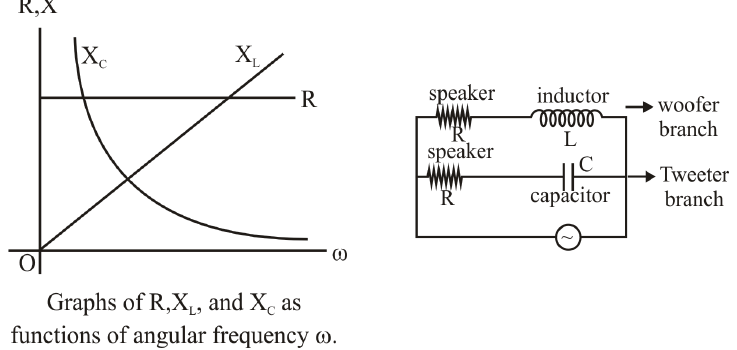
\includegraphics[width=0.7\linewidth]{Score-II - Test 37 (10 Feb 2025)-img/p1phy_q910_stem.png}
\end{center}
\begin{multicols}{2}

\textbf{9.} The rms current in tweeter and woofer can be equal if:-

\begin{qoptions}
\opt{A}{$\omega=\dfrac1{\sqrt{LC}}$}
\opt{B}{$\omega=\sqrt{\dfrac1{LC}-\dfrac{R^2}{4L^2}}$}
\opt{C}{$\omega=\sqrt{\dfrac1{LC}-\dfrac{R^2}{L^2}}$}
\opt{D}{$\omega=\sqrt{\dfrac1{LC}-\dfrac{R^2}{2L^2}}$}
\end{qoptions}

\textbf{10.} The correct graph for $i_{rms}$ versus angular frequency $\omega$ through tweeter and woofer is shown by:-

\begin{center}
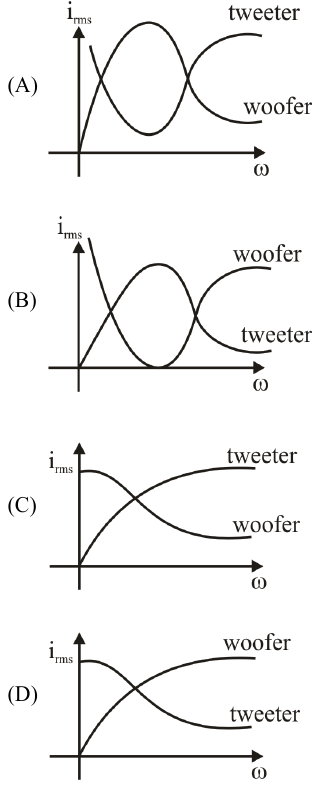
\includegraphics[width=0.65\linewidth]{Score-II - Test 37 (10 Feb 2025)-img/p1phy_q10_graphs.png}
\end{center}

\subsectionhdr{Section-II (i): Paragraph-based Numerical}

\textbf{Paragraph for Questions 1 and 2}

\textbf{Thrust on a Rocket \& Bernoulli's equation.}

Thrust is the force which moves the rocket through the air and through space. Thrust is generated by the propulsion system. An engine does work on a gas or liquid, called a working fluid. Consider a chamber of cross-sectional area A filled with a gas of density $\rho$ at a pressure P as shown in figure. Let there be a small orifice of cross-sectional area A$_0$ at the bottom of the chamber. The speed $v_0$ with which the gas escape through the orifice can be found using Bernouli's equation as
$$P-P_0=\dfrac12\rho\left(v_0^2-v^2\right)$$
Where P$_0$ represents atmospheric pressure just outside the orifice, v is the speed of the following gas inside the chamber and $v_0$ is the speed of gas through orifice. Since the gas density is negligible, pressure variation with height in the chamber can be neglected. (A $\gg$ A$_0$) (Use P = $10\times10^5$ Pa, P$_0$ = $1\times10^5$ Pa, $\rho$ = $0.5\times10^3$ kg/m$^3$, A$_0$ = 0.5 m$^2$)

\begin{center}
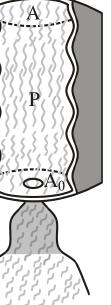
\includegraphics[width=0.5\linewidth]{Score-II - Test 37 (10 Feb 2025)-img/p1phy_n12_rocket.png}
\end{center}

\textbf{1.} The thrust force acting on the rocket due to this will be F $\times10^5$ N. Write value of F.

\textbf{2.} For A $\gg$ A$_0$, the speed of gas through the chamber will be $v_0$ m/s. Find value of $v_0/10$.

\textbf{Paragraph for Questions 3 and 4}

Consider a conducting, uniform, thin hemispherical shell of radius R, which is connected with two wires along its diameter, carrying current I as shown. Neglect field of connecting wire. (I = 2A, R = 1m)

\begin{center}
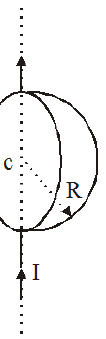
\includegraphics[width=0.4\linewidth]{Score-II - Test 37 (10 Feb 2025)-img/p1phy_n34_hemisphere.png}
\end{center}

\textbf{3.} What is magnetic field due to hemisphere at it's center in $\mu$T?

\textbf{4.} If uniform magnetic field B of magnitude 0.1 T, is applied in direction perpendicular to base of hemisphere, what will be force on it (in N)

\textbf{Paragraph for Questions 5 and 6}

A large 16.0-kg roll of paper with radius R = 18.0 cm rests against the wall and is held in place by a smooth massless axis attached to a rod through the centre of the roll as shown in figure. The moment of inertia of the paper roll about the axis is 0.360 kg$\cdot$m$^2$. The other end of the rod is attached by a frictionless hinge to the wall such that the axis makes an angle of 37\textdegree\ with the wall. The weight of the rod is negligible. The coefficient of kinetic friction between the paper and the wall is $\mu_k=1/3$. A constant vertical force F = 400 N is applied to the paper, and the paper unrolls. (g = 10 m/s$^2$)

\begin{center}
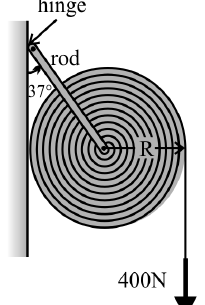
\includegraphics[width=0.55\linewidth]{Score-II - Test 37 (10 Feb 2025)-img/p1phy_n56_paperroll.png}
\end{center}

\textbf{5.} The magnitude of the angular acceleration (in rad/sec$^2$) of the roll is:

\textbf{6.} The magnitude of the tension force (in newton) that the rod exerts on the paper roll as it unrolls is:

\subsectionhdr{Section-II (ii): Non-negative Integer}

\textbf{7.} A circular parallel plate capacitor having plate radius R is charged by means of a cell at time t = 0. The variation of the current through the connecting wires with time is shown in figure. Consider a plane circular area of radius R/2 parallel to the plates and situated symmetrically between them.

\begin{center}
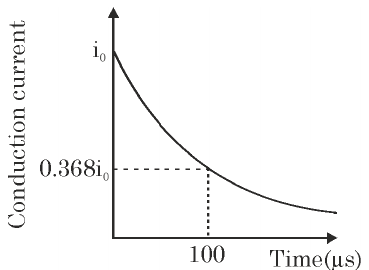
\includegraphics[width=0.65\linewidth]{Score-II - Test 37 (10 Feb 2025)-img/p1phy_n7_currentgraph.png}
\end{center}

Assuming $i_0$ = 5A, the time rate change of electric flux through the area at t = 100 $\mu$s is $\dfrac n2\times10^{11}\dfrac{\text{N-m}^2}{\text{C-s}}$, then the integer closest to n = \_\_\_\_.

\textbf{8.} A spring of spring constant 2000N/m is suspended vertically in earth's gravitational field and a mass of 0.8 kg is hung from it. It is hanging in equilibrium. At t = 0, a force of 72 N starts acting in vertically downward direction. The force ceases to act at $t=\dfrac\pi2$ sec. If the amplitude of resulting SHM (in mm) after that is given by N. Fill value of $\dfrac N{24}$

\textbf{9.} A particle moves along a straight line path such that its magnitude of velocity is given by $v=(3t^2-6t)$ ms$^{-1}$, where t is the time in seconds. If it is initially located at the origin O then determine the magnitude of particle's average speed in time interval from t = 0 to t = 4s

\sectionhdr{PART-2: CHEMISTRY}
\subsectionhdr{Section-I (i): One or more correct}

\textbf{1.} Select correct option among the following statements:

(P) Sol prepared by hydrolysis of FeCl$_3$, colloidal particles get attracted forward anode during electrophoresis.

(Q) A gas with higher critical temperature gets adsorbed to more extent than a gas with lower critical temperature.

(R) On mixing of eosin (acid dye) and haemoglobin (blood), coagulation takes place.

(S) Gold sol is deposited at anode in the electro osmosis process.

(T) CMC value of CH$_3$(CH$_2$)$_8$NH$_3^\oplus$Cl$^\ominus$ will be less than that of CH$_3$(CH$_2$)$_5$COONa.

(U) Brownian motion is independent of nature of colloid but depends on viscosity of solution.

\begin{qoptions}
\opt{A}{PQR}
\opt{B}{QRT}
\opt{C}{RTU}
\opt{D}{QTU}
\end{qoptions}

\textbf{2.} In the given chemical reaction,
$$\text{AgClO}_{3(s)}+[\text P]_{(g)}\xrightarrow{90^\circ\text C}[\text Q]_{(s)}+[\text R]_{(g)}+[\text S]_{(g)\text{(Diatomic)}}$$
Identify [P], [Q], [R] and [S]. if gas [P] can be prepared by dissolving red lead (Pb$_3$O$_4$) in warm hydrochloric acid?

\begin{qoptions}
\opt{A}{[P] = Cl$_2$}
\opt{B}{[Q] = AgCl}
\opt{C}{[R] = ClO$_2$}
\opt{D}{[S] = O$_2$}
\end{qoptions}

\textbf{3.} Correctly matched reaction with their major product.

\end{multicols}
\begin{center}
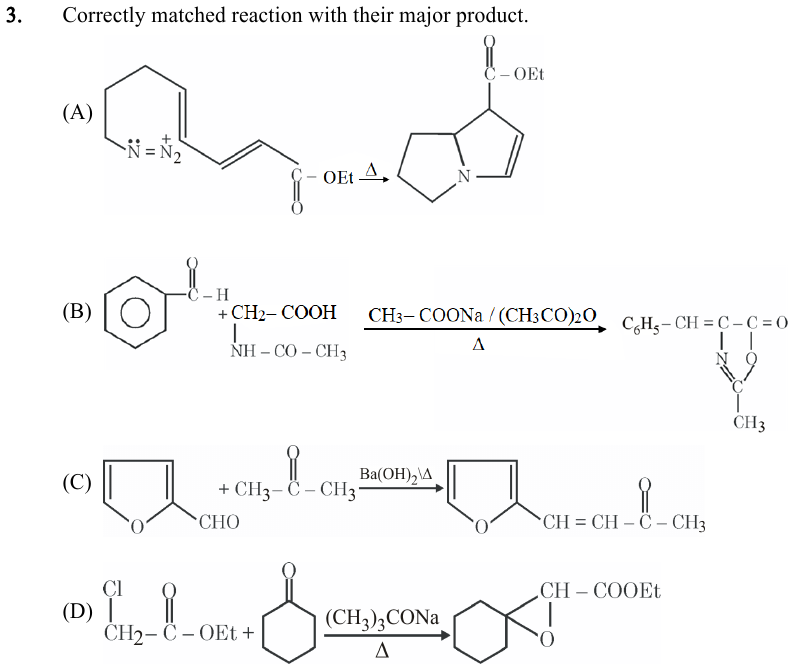
\includegraphics[width=0.85\linewidth]{Score-II - Test 37 (10 Feb 2025)-img/p2chem_q3_reactions.png}
\end{center}
\begin{multicols}{2}

\textbf{4.}

\begin{center}
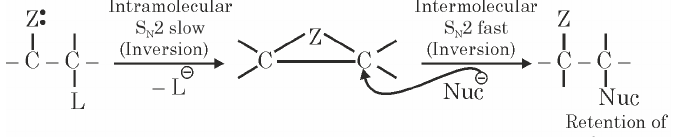
\includegraphics[width=0.95\linewidth]{Score-II - Test 37 (10 Feb 2025)-img/p2chem_q4_mechanism.png}
\end{center}

A common feature of all neighbouring group mechanisms is the formation of a cyclic intermediate. The neighbouring group acting as the nucleophile ($\ddot Z$) is present in the same molecule and is immediately available for the attack, such reactions occur 1000 times faster than comparable internuclear nucleophilic substitution. True statement among the following is/are

\begin{qoptions}
\opt{A}{Rate of acetolysis of 4-methoxybutyl brosylate is nearly 650 times faster than that of n butyl brosylate.}
\opt{B}{2-Bromopropanoic acid is treated with dil. alkali, it gives lactate anion with complete retention of configuration.}
\opt{C}{Rate of acetolysis of trans-2-iodocyclohexyl brosylate is $1.7\times10^6$ times slower than that of its cis isomer.}
\opt{D}{Optically active erythro-3-Bromo-2-butanol react with HBr with retention of configuration to give Meso-dibromide.}
\end{qoptions}

\textbf{5.} The following graph is given, between total energy and distance between the two nuclei for species H$_2^+$, H$_2$, He$_2^+$, \& He$_2$, which of the following statement/s is incorrect:

\begin{center}
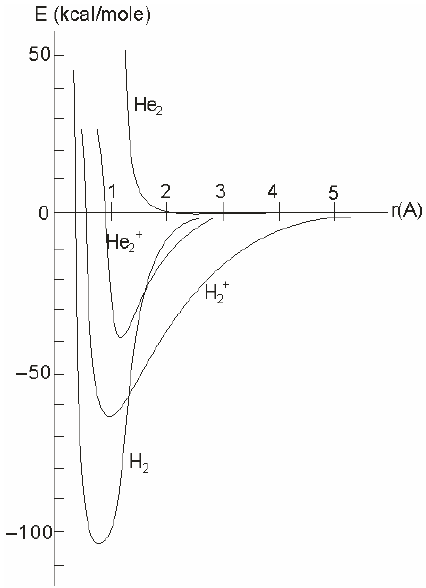
\includegraphics[width=0.75\linewidth]{Score-II - Test 37 (10 Feb 2025)-img/p2chem_q5_energygraph.png}
\end{center}

\begin{qoptions}
\opt{A}{He$_2^+$ is more stable than H$_2^+$}
\opt{B}{Bond dissociation energy of H$_2^+$ is more than bond dissociation energy of He$_2^+$}
\opt{C}{Since bond orders of He$_2^+$ and H$_2^+$ are equal hence both will have equal bond dissociation energy.}
\opt{D}{Bond length of H$_2^+$ is less than bond length of H$_2$}
\end{qoptions}

\textbf{6.} Consider two 0.1 M solutions of two solutes X \& Y in the same solvent. The solute X dimerises in solution while solute Y undergoes trimerisation in solution \& their degree of dimerisation \& trimerisation are 0.8 \& 0.6 respectively then the correct statement(s) among the following is/are:

\begin{qoptions}
\opt{A}{The boiling point of solution of 'X' will be higher than that of 'Y'.}
\opt{B}{The freezing point of solution 'X' will be higher than that of 'Y'.}
\opt{C}{The freezing point of solution 'X' and solution 'Y' are same.}
\opt{D}{Due to association of solute 'X' \& 'Y' in solutions, the observed colligative property is less than that of calculated colligative property for both these solutions.}
\end{qoptions}

\subsectionhdr{Section-I (ii): Single Correct}

\textbf{Paragraph for Questions 7 and 8}

Cast iron is prepared from haematite. The ore is roasted to remove the volatile impurities. During roasting the mass becomes porous. Iron in the form of ferrous oxide is converted to ferric oxide. Finally ferric oxide is mixed with coke and heated in a blast furnace. Pig iron is formed and is casted in the desired shape.

\textbf{7.} Carbon in cast iron can be represented by -

\begin{qoptions}
\opt{A}{FeC}
\opt{B}{Fe$_3$C}
\opt{C}{FeC$_3$}
\opt{D}{Fe$_2$C}
\end{qoptions}

\textbf{8.}

\begin{center}
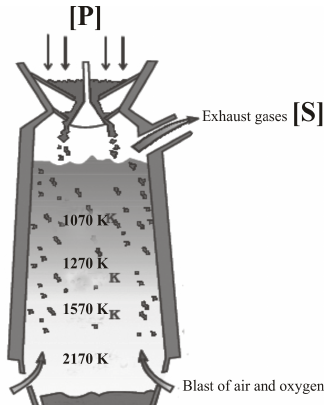
\includegraphics[width=0.85\linewidth]{Score-II - Test 37 (10 Feb 2025)-img/p2chem_q8_furnace.png}
\end{center}

Identify [P], [Q], [R] and [S] in above metallurgical diagram -

\begin{qoptions}
\opt{A}{[Fe$_2$O$_3$ + Silicate + coke], [Pig iron], [Slag], [SO$_2$, CO$_2$]}
\opt{B}{[FeS + Silicate + coke], [Slag], [Pig iron], [CO, CO$_2$]}
\opt{C}{[Fe$_2$O$_3$ + lime stone + coke], [Slag], [Cast iron], [CO, CO$_2$]}
\opt{D}{[Fe$_2$O$_3$ + lime stone + coke], [Solid waste], [Pig iron], [CO, CO$_2$]}
\end{qoptions}

\textbf{Paragraph for Questions 9 and 10}

\begin{center}
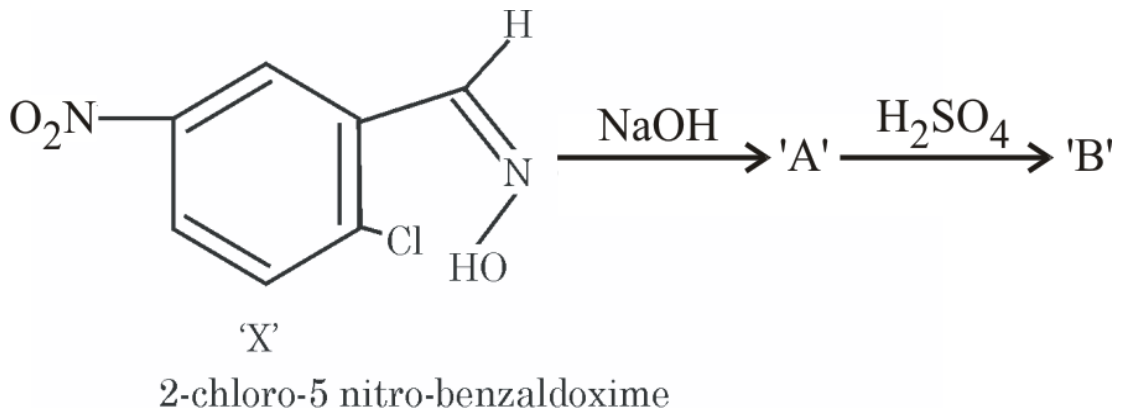
\includegraphics[width=0.85\linewidth]{Score-II - Test 37 (10 Feb 2025)-img/p2chem_q910_stem.png}
\end{center}

\textbf{9.} Incorrect statement among the following is

\begin{qoptions}
\opt{A}{Out of two isomers of 'X' only, anti isomer on treatment with NaOH readily give ring closure.}
\opt{B}{Rate of conversion of 'X' to A could be increased in case of its flouro derivative.}
\opt{C}{B compound is \raisebox{-0.4\height}{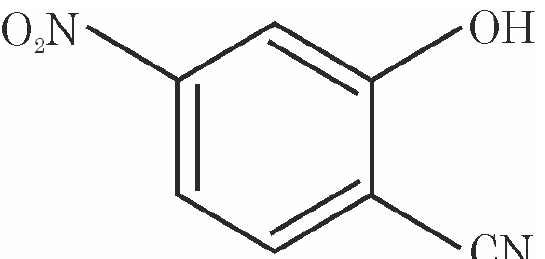
\includegraphics[width=0.32\linewidth]{Score-II - Test 37 (10 Feb 2025)-img/p2chem_q9_optC.png}}}
\opt{D}{During formation of A to B, rearrangement takes place.}
\end{qoptions}

\textbf{10.} Correct statement out of the following:

\end{multicols}
\begin{center}
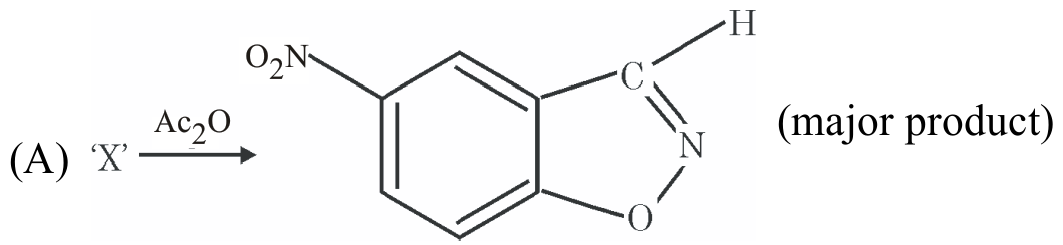
\includegraphics[width=0.85\linewidth]{Score-II - Test 37 (10 Feb 2025)-img/p2chem_q10_optA_full.png}
\end{center}
\begin{center}
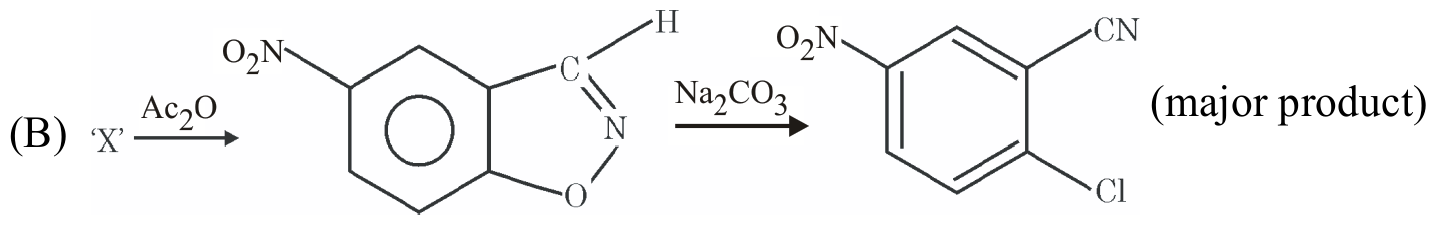
\includegraphics[width=0.95\linewidth]{Score-II - Test 37 (10 Feb 2025)-img/p2chem_q10_optB_full.png}
\end{center}
\begin{multicols}{2}

\noindent(C) $'X'\xrightarrow{\text{Ac}_2\text O}P\xrightarrow{\text{Na}_2\text{CO}_3}Y'$. Step P to Y involve Meisenheimer complex

\end{multicols}
\begin{center}
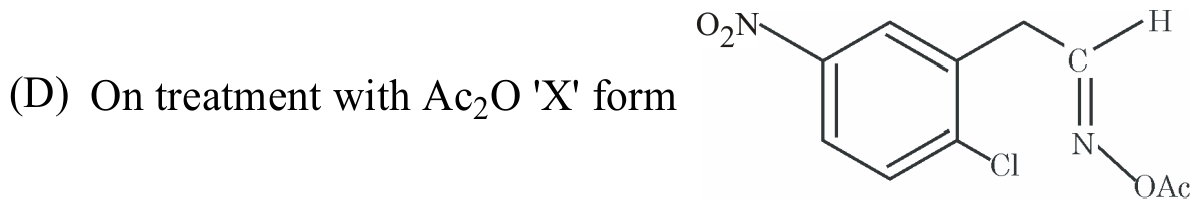
\includegraphics[width=0.8\linewidth]{Score-II - Test 37 (10 Feb 2025)-img/p2chem_q10_optD_full.png}
\end{center}
\begin{multicols}{2}

\subsectionhdr{Section-II (i): Paragraph-based Numerical}

\textbf{Paragraph for Questions 1 and 2}

Values of $\Delta_o$ (in eV/ion) for some transition metal complexes are:

Co$^{3+}$ 3.501 in Co(NO$_2$)$_6^{3-}$

Co$^{2+}$ 2.242 in Co(NO$_2$)$_6^{4-}$

The t$_{2g}$ orbitals are lowered by $\dfrac25\Delta_o$, and the e$_g$ orbitals are raised by $\dfrac35\Delta_o$. You are given the complex ions: Co(NO$_2$)$_6^{3-}$ and Co(NO$_2$)$_6^{4-}$. Assume all complexes can be either in the high spin (H.S.) state or the low spin (L.S.) state.

\textbf{1.} Calculate the wavelength, $\lambda$ (in nm), which is absorbed by the complex Co(NO$_2$)$_6^{3-}$ for d-d transition.

\textbf{2.} Calculate the magnitude of crystal field stabilization energy, CFSE in kJ/mole, assuming given complex Co(NO$_2$)$_6^{4-}$ is a high spin complex ion. (Take charge on 1e$^-$ = $-1.602\times10^{-19}$ C, Avogadro number = $6.022\times10^{23}$)

\textbf{Paragraph for Questions 3 and 4}

\begin{center}
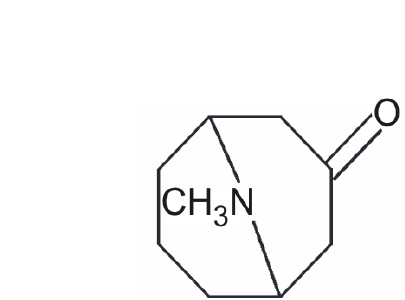
\includegraphics[width=0.3\linewidth]{Score-II - Test 37 (10 Feb 2025)-img/p2chem_stem34_bicyclic.png}
\end{center}

K + heat $\to$ L(C$_9$H$_{15}$N)

L + CH$_3$I, then Ag$_2$O $\to$ M(C$_{10}$H$_{19}$ON)

M + heat $\to$ N(C$_{10}$H$_{17}$N)

N + CH$_3$I, then Ag$_2$O $\to$ O(C$_{11}$H$_{21}$ON)

O + heat $\to$ P(C$_8$H$_{10}$)

P + Br$_2$ $\to$ Q(C$_8$H$_{10}$Br$_2$)

Q + (CH$_3$)$_2$NH $\to$ R(C$_{12}$H$_{22}$N$_2$)

R + CH$_3$I, then Ag$_2$O $\to$ S(C$_{14}$H$_{30}$O$_2$N$_2$)

S + heat $\to$ T(C$_8$H$_8$)

\textbf{3.} T reacts with Na metal (excess) to give a stable compound U. Number of $\pi$ bonds present in T if a number of $\pi$ electrons present in U if b then find out $|a-b|$.

\textbf{4.} Index of hydrogen deficiency in structure `L' is

\textbf{Paragraph for Questions 5 and 6}

Consider the thermodynamic data:

$E^0_{\text{Zn}^{2+}/\text{Zn}}=-0.76$, $E^0_{\text{Fe}^{2+}/\text{Fe}}=-0.44\text V$

$E^0_{\text{Cu/Cu}^{2+}}=-0.34\text V$, $E^0_{\text{Ag/Ag}^\oplus}=-0.8\text V$

$\text{Hg}_2\text{Cl}_{2(s)}+2e^\ominus\to2\text{Hg}_{(l)}+2\text{Cl}^-$; $E^o=0.27\text V$

$\text{Hg}_{2(aq)}^{2+}\to2\text{Hg}_{(aq)}^{2+}+2e^\ominus$; $E^o=-0.92\text V$

$2\text{Hg}_{(l)}\to\text{Hg}_2^{2+}+2e^\ominus$; $E^o=-0.79\text V$

$\text{Hg}_2\text{Cl}_{2(s)}+2e^\ominus\to2\text{Hg}_{(l)}+2\text{Cl}^\ominus_{\text{(saturated)}}$; $E^\circ=0.24\text V$

$\text{Cl}_2+2e^\ominus\to2\text{Cl}^\ominus_{(aq)}$; $E^\circ=1.36\text V$

$\dfrac{2.303RT}F=0.06$

\textbf{5.} How many of the statement(s) is/are correct?

(i) $2\text{Ag}_{(s)}+2\text{HCl}_{(aq)}\to2\text{AgCl}_{(s)}+\text H_2\uparrow$ is spontaneous in standard conditions.

(ii) $\text{Zn}+\text H_2\text{SO}_{4(aq.)}\to\text{ZnSO}_4+\text H_2\uparrow$ is spontaneous in standard conditions.

(iii) $\text{Cu}+\text H_2\text{SO}_{4(aq.)}\to\text{CuSO}_4+\text H_2\uparrow$ is spontaneous in standard conditions.

(iv) $2\text{Ag}+\text{Zn}^{2+}_{(aq)}\to2\text{Ag}^\oplus_{(aq)}+\text{Zn}_{(s)}$ is spontaneous in standard conditions.

(v) For electrolysis, only D.C. current is suitable not A.C. current

(vi) At negative electrode, oxidation takes place in both galvanic \& electrolytic cell

(vii) For the galvanic cell constructed with hydrogen electrode \& chlorine electrode, salt bridge may not be necessary when electrolyte is HCl.

\textbf{6.} How many of the following statement(s) is/are correct

(i) $E^0_{\text{Hg}^{2+}/\text{Hg}}=0.855\text V$

(ii) $E^0_{\text{Hg}^{2+}/\text{Hg}}=-0.855\text V$

(iii) Standard reduction potential of calomel electrode is 0.27 V.

(iv) Oxidation potential of calomel electrode at 1M KCl is $-0.27$ V.

(v) Reduction potential of calomel electrode at 0.1N KCl is 0.33 V.

(vi) K$_{SP}$ of Hg$_2$Cl$_2$ is nearly $10^{-17.33}$.

\subsectionhdr{Section-II (ii): Non-negative Integer}

\textbf{7.} Boric acid $\xrightarrow[\text{Heat}]{\text{Strong}}$X$\xrightarrow[\Delta]{\text C/\text{Cl}_2}$Y

Y + LiAlH$_4\to$'A'$\xrightarrow[\text{low temp}]{\text{NH}_3}$'B'$\xrightarrow[200^\circ\text C]\Delta$'C'

\hspace{1.5em}$\downarrow$\,\,$\xrightarrow[150^\circ\text C]{\text{NH}_4\text{Cl}}$'D'$\xrightarrow{\text{NaBH}_4}$C$\xrightarrow{3\text{HCl}}$'E'

Identify the correct statement/s for the above sequence of the reactions

\begin{qoptions}
\opt{A}{H$_3$BO$_3$ is weak mono acidic Bronsted acid}
\opt{B}{H$_3$BO$_3$ can't be titrated directly with NaOH by using Phenophtathalein indicator}
\opt{C}{H$_3$BO$_3$ is a weak Lewis acid}
\opt{D}{Acidic strength of H$_3$BO$_3$ solution is increases on addition of catecol.}
\opt{E}{`X' on heating with metal oxide, gives metal metaborates}
\opt{F}{`A' is treated with (CH$_3$)$_3$B gives B$_2$(CH$_3$)$_6$ as a product}
\opt{G}{In `C' and `E', boron has sp$^2$ and sp$^3$ hybridization respectively}
\opt{H}{`C' is more reactive than C$_6$H$_6$ towards addition reactions}
\opt{I}{`E' has planar structure}
\opt{J}{`D' has 2p$\pi$-2p$\pi$ backbonding.}
\end{qoptions}

\textbf{8.} Identify number of reactions in which given major product is correct

\end{multicols}
\begin{center}
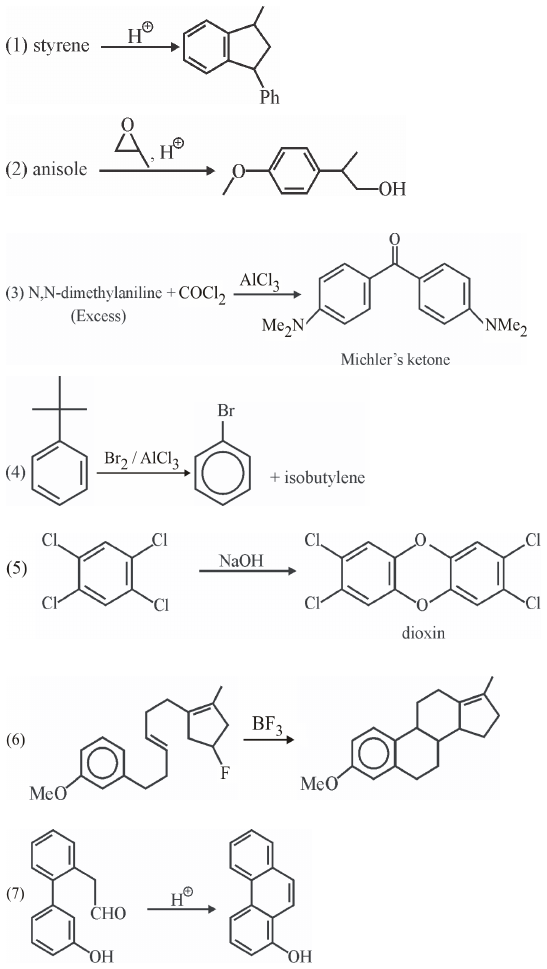
\includegraphics[width=0.62\linewidth]{Score-II - Test 37 (10 Feb 2025)-img/p2chem_n8_reactions.png}
\end{center}
\begin{multicols}{2}

\textbf{9.} 10 moles of an ideal gas is participating in the carnot cycle as shown in the figure.

\begin{center}
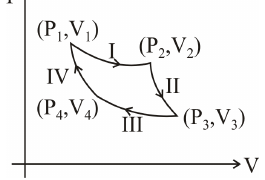
\includegraphics[width=0.55\linewidth]{Score-II - Test 37 (10 Feb 2025)-img/p2chem_n9_carnot.png}
\end{center}

Step-I: Isothermal reversible expansion with absorption of q$_1$ amount of heat

Step-II: Adiabatic reversible expansion

Step-III: Isothermal reversible compression with rejection of q$_2$ amount of heat

Step-IV: Adiabatic reversible compression

Given v$_1$, v$_2$, v$_3$, v$_4$ are the volumes of gases in the corresponding stages, then calculate the value of $nR\ln\dfrac{v_2v_4}{v_1v_3}$?

\sectionhdr{PART-3: MATHEMATICS}
\subsectionhdr{Section-I (i): One or more correct}

\textbf{1.} A and B are two $n\times n$ matrices such that $\det(A)\ne0$, $A+B=(AB)^2$ and $BAB=A+I$. Choose the correct option(s).

\begin{qoptions}
\opt{A}{$A^{-1}=(A^4-I)$}
\opt{B}{$B^5-A^5=A+B$}
\opt{C}{$A^9=A^4+A+I$}
\opt{D}{$A^2B^2=BA^2B$}
\end{qoptions}

\textbf{2.} Let $d(x,[a,b])=\min\{|x-y|:a\le y\le b\}$. A function $f:\mathbb R\to[0,1]$ is defined by
$$f(x)=\dfrac{d(x,[0,1])}{d(x,[0,1])+d(x,[2,3])}\text{,}$$
then which of the following is \textbf{not} correct?

\begin{qoptions}
\opt{A}{the function f is one-one}
\opt{B}{the function f is onto}
\opt{C}{the function f is a bijection}
\opt{D}{the function f is odd}
\end{qoptions}

\textbf{3.} A parabola touches x-axis and the line $y=x$ respectively at points $(1,0)$ and $(1,1)$, then

\begin{qoptions}
\opt{A}{slope of directrix of the parabola is $-2$}
\opt{B}{slope of axis of the parabola is $\dfrac13$}
\opt{C}{focus of the parabola is at the point $\left(\dfrac25,\dfrac45\right)$}
\opt{D}{focus of the parabola is at the point $\left(\dfrac35,\dfrac15\right)$}
\end{qoptions}

\textbf{4.} Equation of curve passing through $(3,4)$ and satisfying the differential equation, $y\left(\dfrac{dy}{dx}\right)^2+(x-y)\dfrac{dy}{dx}-x=0$ can be

\begin{qoptions}
\opt{A}{$x^2+y^2=25$}
\opt{B}{$x^2-y^2+7=0$}
\opt{C}{$xy=12$}
\opt{D}{$x-y+1=0$}
\end{qoptions}

\textbf{5.} Let $x,y,z\in\{1,2,3,4,5,6,7,8,9\}$ such that
$$\sqrt{\underbrace{xxxx\ldots xx}_{\text{``2000'' times}}-\underbrace{yyyy\ldots y}_{\text{``1000'' times}}}=\underbrace{zzzz\ldots zz}_{\text{``1000'' times}}$$
then

\begin{qoptions}
\opt{A}{$x+y+z$ can be 6}
\opt{B}{$x+z$ can be 18}
\opt{C}{$x+y+z$ can be 18}
\opt{D}{x can be 9}
\end{qoptions}

\textbf{6.} Let z, z$_1$, z$_2$ be three distinct complex numbers and $\text{Im }z\ne0$. If $(z^2+1)(\bar z^2+1)=\left(1+\left(\dfrac{z+\bar z}2\right)^2\right)^2$ and $z_1=i$, $z_2=-i$, $(i=\sqrt{-1})$ then (If $z=a+ib$ then $\bar z=a-ib$, $a,b\in\mathbb R$)

\begin{qoptions}
\opt{A}{$|z|<3$}
\opt{B}{Locus of z may be an ellipse}
\opt{C}{Locus of z may be a hyperbola}
\opt{D}{$|z_1-z_2|+|z_1-z|+|z_2-z|=2\sqrt2+2$}
\end{qoptions}

\subsectionhdr{Section-I (ii): Single Correct}

\textbf{Paragraph for Questions 7 and 8}

A first order first degree differential equation can be written in the exact differential form which can be easily integrated. Example: $xdy+ydx=d(xy)$, $\dfrac{xdy+ydx}{xy}=d(\ln xy)$, etc. Now answer the following using this exact differential concept or otherwise.

\textbf{7.} The curve C which passes through $(1,1)$ and satisfies the differential equation $(2x^2y-2y^4)dx+(2x^3+3xy^3)dy=0$ is given by, $\alpha\ln|x|+\beta\ln|y|+\dfrac{y^3}{x^2}=\gamma$, then $(\alpha+\beta+\gamma)$ is equals to

\begin{qoptions}
\opt{A}{3}
\opt{B}{4}
\opt{C}{5}
\opt{D}{6}
\end{qoptions}

\textbf{8.} A curve $y=f(x)$ passing through the point $\left(\dfrac12,\dfrac14\right)$ satisfies the differential equation, $\dfrac xy\dfrac{dy}{dx}=\dfrac{3x^2-y}{2y-x^2}$ is a conic whose length of latus rectum is

\begin{qoptions}
\opt{A}{1}
\opt{B}{2}
\opt{C}{3}
\opt{D}{4}
\end{qoptions}

\textbf{Paragraph for Questions 9 and 10}

a$_1$, a$_2$, a$_3$ are three consecutive terms of an increasing A.P., where a$_1$ and a$_2$ are prime numbers such that their sum is minimum possible odd prime number.

Urn-1: Contains a$_1$ red and a$_3$ green balls

Urn-2: Contains a$_2$ red and a$_2$ green balls

Urn-3: Contains a$_3$ red and a$_1$ green balls

P(i) represents the probability of choosing i$^{th}$ urn and P(R) represents probability of choosing red ball and similarly P(G) represents the probability of choosing green ball.

\textbf{9.} If $P(i)\propto i^2$ and one ball is drawn from one of these urns then P(R) is equal to

\begin{qoptions}
\opt{A}{$\dfrac67$}
\opt{B}{$\dfrac{17}{42}$}
\opt{C}{$\dfrac{23}{42}$}
\opt{D}{$\dfrac{25}{42}$}
\end{qoptions}

\textbf{10.} If $P(i)=1/3$ for all $i=1,2,3$ and 2 balls are drawn randomly from one of these urns then the chance of drawing balls of different colours is

\begin{qoptions}
\opt{A}{$\dfrac49$}
\opt{B}{$\dfrac59$}
\opt{C}{$\dfrac79$}
\opt{D}{$\dfrac89$}
\end{qoptions}

\subsectionhdr{Section-II (i): Paragraph-based Numerical}

\textbf{Paragraph for Questions 1 and 2}

A ten-sided regular polygon is inscribed in a circle $|z|=1$, A$_{10}$, A$_1$, A$_2$, ....., A$_9$ be its vertices in anticlockwise with A$_{10}=(1,0)$. G$_1$ is centroid of $\triangle$A$_1$A$_4$A$_8$, G$_2$ be centroid of $\triangle$A$_2$A$_6$A$_9$ and G$_3$ be centroid of $\triangle$A$_3$A$_5$A$_7$. P is centroid $\triangle$G$_1$G$_2$G$_3$. If `O' is the centre of circle.

\textbf{1.} Angle $\angle$POA$_1$ is equal to $k\pi$, then k is equal to

\textbf{2.} $90\times|OP|$ is equal to

\textbf{Paragraph for Questions 3 and 4}

If
$$\resizebox{\linewidth}{!}{$L=\displaystyle\lim_{x\to0}\dfrac{\sqrt{1+x^2}\tan\sin\tan^{-1}x+2\sqrt{1-x^2}\sin\tan\sin^{-1}x-3x}{x^p}$}$$
exists finitely and takes non-zero value $(p\ge2,p\in\mathbb N)$, then

\textbf{3.} The value of p is

\textbf{4.} The value of $60|L|$ is

\textbf{Paragraph for Questions 5 and 6}

From the set of n number $\{1,3,5,\ldots,2n-1\}$ five consecutive numbers are removed and the mean of remaining numbers is $\dfrac{393}5$.

\textbf{5.} The value of n is

\textbf{6.} The mean of removed numbers is

\subsectionhdr{Section-II (ii): Non-negative Integer}

\textbf{7.} Consider a function $f(x)$ which satisfies $f'(x)-\tan x.f(x)=\displaystyle\int_{-\pi/6}^{\pi/6}f(x)\,dx\ \ \forall\ x\in\left(-\dfrac\pi2,\dfrac\pi2\right)$ and $f(0)=1$. The value of $\left(f\left(\dfrac\pi3\right)-\sqrt3\ln3\right)$ is

\textbf{8.} Consider the following three planes

$p_1: 2x+y+z=1$

$p_2: x-y+z=2$

$p_3: kx-y+3z=5$

The three planes intersect each other at point R on XOY plane and at the point S on YOZ plane `O' is Origin. If the coordinates of point `P' situated at minimum distance from point 'O' on the RS are $(\alpha,\beta,\gamma)$. Then the value of $\left(\dfrac\alpha2-180\beta+2\gamma\right)$ is a three digit number abc then $a+b-c$ is equal to

\textbf{9.} Let $n\in\mathbb N$, $A^n=\begin{bmatrix}2&1\\1&0\end{bmatrix}^n=\begin{bmatrix}a_{11}(n)&a_{12}(n)\\a_{21}(n)&a_{22}(n)\end{bmatrix}$. If $\displaystyle\lim_{n\to\infty}\dfrac{a_{12}(n)}{a_{22}(n)}=\ell$, where $\ell^2=\sqrt a+\sqrt b$ $(a,b\in\mathbb N,a>b)$. Then $(a+b)$ is equal to

\end{multicols}
\end{document}
